\begin{IEEEbiography}[{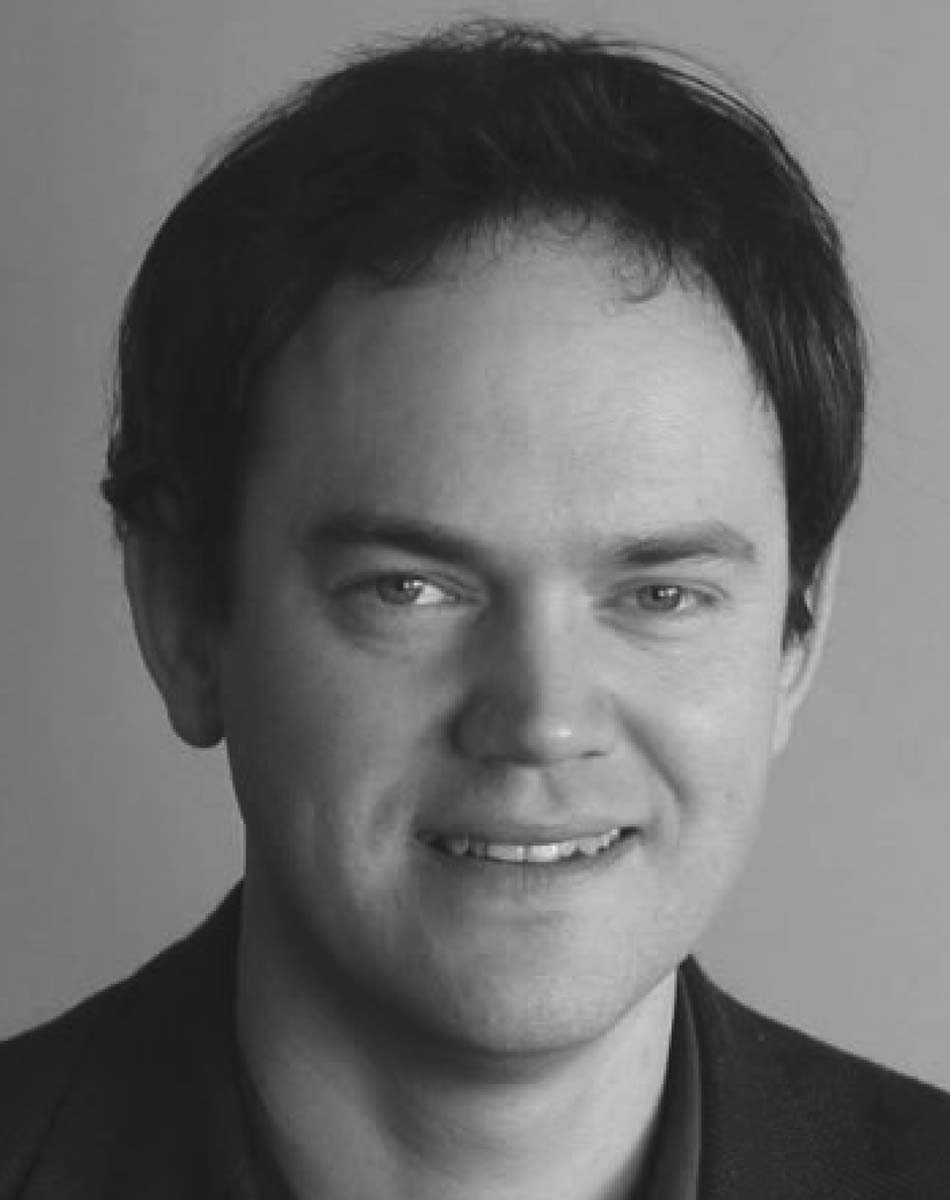
\includegraphics[width=1in,height=1.25in,clip,keepaspectratio]{Godsill.jpg}}]{Simon Godsill} is Professor of Statistical Signal Processing in the Engineering Department at Cambridge University and a Professorial Fellow and tutor at Corpus Christi College Cambridge.

He coordinates an active research group in Signal Inference and its Applications within the Signal Processing and Communications Laboratory at Cambridge, specialising in Bayesian computational methodology, multiple object tracking, audio and music processing, and financial time series modeling. A particular methodological theme over recent years has been the development of novel techniques  for optimal Bayesian filtering and smoothing, using Sequential Monte Carlo or Particle Filtering methods.

Prof. Godsill has published extensively in journals, books and international conference proceedings. He was technical chair of the IEEE NSSPW workshop in 2006 on sequential and nonlinear filtering methods, was Technical Chair for Fusion 2010 in Edinburgh, and has been on the conference panel for numerous other conferences and workshops. Prof. Godsill has served as Associate Editor for IEEE Tr. Signal Processing and the journal Bayesian Analysis. He was Theme Leader in Tracking and Reasoning over Time for the UK�s Data and Information Fusion Defence Technology Centre (DIF-DTC) and Principal Investigator on grants funded by the EU, EPSRC, QinetiQ, General Dynamics, MOD, Microsoft UK, Citibank and Mastercard. In 2009-10 he was co-organiser of an 18 month research program in Sequential Monte Carlo Methods at the SAMSI Institute in North Carolina. He is a Director of CEDAR Audio Ltd. (which has received a technical Oscar for its audio processing work), and Input Dynamics Ltd., both companies which use his research work in the audio area.   


\end{IEEEbiography} 